\chapter{Approximating Type Stability Statically}\label{chap:approx}

\lstset{language=julia}

\paragraph{Plan of attack}
\begin{enumerate}

\item
Inferring type stability versus inferring types

\item
Method: Using Julia's built-in type inferencer to approximate type stability.

\item
Basic algorithm and its features.

- Corner cases, termination, fuel.

- Limitations: incompleteness and unsoundness.

- Relation to Julia subtyping.

\item
Dealing with unbounded existentials / Any's: the types DB idea.

\item
Implementation.

\item
Evaluation: results on 10 popular Julia packages.

- Processing Julia modules: pitfalls and workarounds.

\end{enumerate}

Chapters~\ref{sec:empirical} and~\ref{sec:jules} consider type stability as it
relates to program \emph{execution}: chapter~\ref{sec:empirical} analyzes Julia
VM state after test suites ran, and chapter~\ref{sec:jules} models a
type-specializing just-in-time compiler that does its main job at the run time.
In this chapter, I set to approximate the property of type stability for
arbitrary Julia code statically, without running the code in question.

\paragraph{Note on Dropping Type Groundedness} It turns out that attempts to
infer type groundedness statically fail fast: this is a too low-level of
notion requiring us to reason on a level of intermediate representation, and at
that level precision gets lost very fast. The good news is that, as we learned
in~\chapref{sec:jules}, type groundedness is based off calling type-stable
API, so being able to provide such API should be enough for a careful client.
Therefore, in this chapter we focus on analyzing type stability of methods, and
leave type groundedness off.

\section{Inferring Type Stability versus Inferring Types}
% \section{Inferring Types(tability)} ha-ha

Explaining my method to infer type stability requires a definition for it.
So far, I approached the definition twice: informally
in~\ref{ssect:ts-informal} and formally in~\ref{sec:stability-formal}.
The original informal
definition does not take into account the distinction between concrete and
abstract types: using this loophole, any code can be declared type stable
because it is always ``possible to predict the type of the output'' as \c{Any}.
Building upon the formal definition (that does acknowledge the distinction
between abstract and concrete types)
we provide another informal definition to explain intuitions behind this
chapter.
\begin{definition}[Type Stability, Informally]
  A Julia method is called \emph{type stable} if for any concrete type of the
  input, it is possible to infer a concrete type of the return value.
\end{definition}

A natural idea for inferring type stability in Julia would be to formulate it as
a forward static analysis: being an abstract or concrete type is one bit of
information that has a known value at the input (concrete) and should be
propagated to the output, possibly changing on the way.

To test the static analysis idea, consider a positive example first: the
identity function.
% TODO: there's a weird break in the listing near page break (see PDF)
\begin{lstlisting}
  function id(x)
    x
  end
\end{lstlisting}
%
It is straightforward to infer that, given any concrete input type, the return
value is also concretely typed: the one bit of information carries over to the
result in one step.

Another example, the increment function, shows that the task becomes unwieldy fast.
%
\begin{lstlisting}
  function inc(x)
    x + 1
  end
\end{lstlisting}
%
Concreteness of the result returned by \c{inc} depends on the same property of
the result of the call to \c{+}. In turn, the property of the return type of
\c{+} depends on which \c{+} method Julia will dispatch to at the run time.
There are about two hundreds method implementations of \c{+} in the standard
library alone, and packages add more. Some of those methods are type stable
(e.g. \c{+(::Int64,::Int64)}), and some of them not (e.g.
\lstinline|+(::Rational{Bool},::Rational{Bool}|)
\footnote{%
  The reason for the
  \c{+(::Rational\{Bool\},::Rational\{Bool\})} method to be not type
  stable is not important, but in the nutshell, Julia has made a questionable
  design decision about the return type of \c{{+}(::Bool,::Bool)}, which in the
  current implementation is \c{Int}
  (see discussion \url{https://github.com/JuliaLang/julia/issues/19168}),
  and when adding two rational numbers with boolean components, depending on the
  values of the summands, you get back either \c{Rational\{Bool\}} or
  \c{Rational\{Int\}}.}
).
Therefore,
to infer the property of interest, in general,
we need to predict which methods are selected at the run time.

The \c{inc} example shows that inferring type stability of Julia code
requires
reasoning about which methods will be called to at the run time, which, in a
language with dynamic dispatch, leads
to reasoning about the \emph{types} of intermediate values, rather than only
the concreteness bit. But if we had a tool to compute typing information
beforehand, we would not need to build a special purpose analysis for type
stability: it suffices to ask the tool to tell the type of the return value and
check if that type is concrete. The observation of interactions between type
stability and type inference can be formulated as the following conjecture.

\begin{conjecture}
Inferring type stability of a Julia method statically is no easier than doing type
inference over that method.
\end{conjecture}

A full type inference algorithm would be enough for checking type stability of
Julia code. Should we build one from scratch? There are two reasons to do
otherwise.
\begin{enumerate}

  \item It is not clear that typing Julia as is can yield any meaningful result
  (more on this see~\cite{Chung23}).

  \item Julia already has a type inference engine built in. We modelled this
        engine as a black box in~\chapref{chap:jules}. If we end up with a
        custom algorithm to infer types and analyze type stability based on it,
        our results may diverge from Julia's.
\end{enumerate}

\section{An Algorithm To Approximate Type Stability}

If our predictions for type stability are to align with the Julia
implementation, our analysis should closely model what happens at the run time,
as described in~\chapref{chap:jules}. The type-specializing JIT-compiler
from~\chapref{chap:jules} makes optimization decisions based on \emph{concrete
  input types} with the help of Juila's type inference engine. Our algorithm for
approximating these decisions statically considers all (or as many as
possible) allowed concrete input types of a method ---~\figref{fig:infer-ts}.

\begin{figure}
  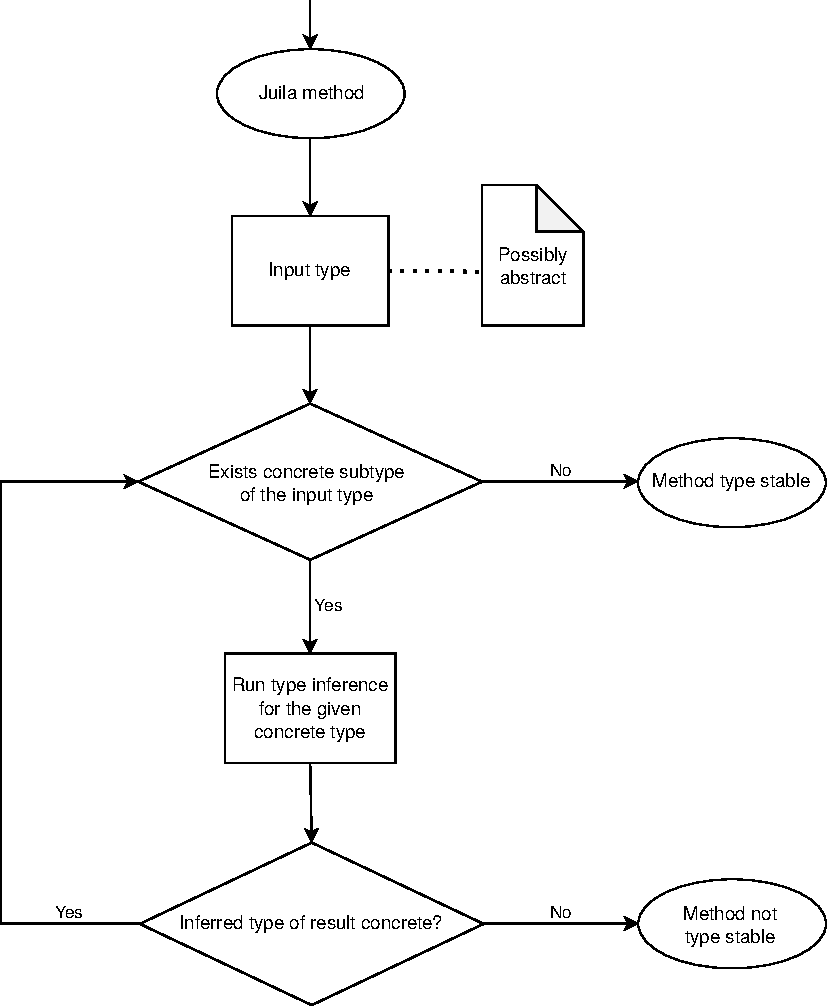
\includegraphics{figs/infer-ts.pdf}
  \caption{Inferring type stability of a Juila method}%
  \label{fig:infer-ts}
\end{figure}


Let us consider every step of the algorithm described
on~\figref{fig:infer-ts} and show its meaning using an example.
The list below also assigns the numbers to each step in our
\begin{enumerate}

  \item The input of the algorithm is a Julia method. Methods in Julia are
  represented by runtime objects of type \c{Method} and can be manipulated as
  all other objects (e.g. stored in collections, responding to field accesses, etc.).

  For example, consider the \c{length} from the Julia's standard library. We can
  get the corresponding \c{Method} object using the standard \c{@which} macro
  applied to an application of the \c{length} method. This can be done in the
  Julia REPL (signified by the \texttt{julia>} prefix).
\begin{verbatim}
  julia> @which length([1,2,3])
  length(a::Array) in Base at array.jl:215
\end{verbatim}

  The output shows that the given \c{length}-call will dispatch to the
  method defined in the \texttt{Base} module (Julia-speak for the standard
  library). The output also shows the location of the method in the
  standard library and, most importantly for us, the signature of the
  method. In fact, what we see here is a pretty-printed representation of
  the \c{Method} object representing a particular Julia method.

  \item The first task of the algorithm is to get the input type of the given
  method. This is possible through querying the \c{sig} field of the method object.

  Building on the example above, we can get the signature of the \c{length}
  method as follows:
\begin{verbatim}
  julia> m = @which length([1,2,3]);

  julia> m.sig
  Tuple{typeof(length), Array}
\end{verbatim}

  A signature of a method will usually have the special singleton function
  type (\c{typeof(...)}) as the first component, and the rest is (easy to
  convert to) the type of the input --- an $n$-tuple. In this example, the type of
  the input is 1-tuple, consisting of the existential array type
  \c{Array\{T, N\}\ where T where N} abbreviated simply as \c{Array}\footnote{%
A user can always look under the abbreviation using the \c{dump} function:
\begin{verbatim}
  julia> dump(Array)
  UnionAll
    var: TypeVar
      name: Symbol T
      lb: Union{}
      ub: Any
    body: UnionAll
      var: TypeVar
        name: Symbol N
        lb: Union{}
        ub: Any
      body: Array{T, N} <: DenseArray{T, N}
\end{verbatim}
}.

  \item The input type can be either concrete, which, in Julia, means there may
  be no proper subtypes of that type, or abstract. Still, the choice on the
  step 3 will enter the loop at least once, because if the input type is
  concrete, the check holds once trivially (e.g.\ there is exactly one concrete
  subtype of the concrete type \c{Int} --- it is \c{Int} itself).

  If the input type is abstract, we need a subprocess enumerating all concrete
  subtypes of it. We discuss an implementation for this below but it suffices to
  treat is as a black box for now. % TODO: ref to subtyping section?

  In the case of the \c{length} method, the input type, \c{Array}, is abstract
  because it is an existential type.

  \item Running type inference for a given method and a given concrete type is
  done through calling the Julia's standard \c{code_typed} function.
\end{enumerate}
